\chapter{Student's t-Distribution ($X \sim t_\nu$) \cite{ism-1,wiki/Student_t-distribution}}\label{Student's t-Distribution}

\begin{table}[H]
    \begin{minipage}{0.49\linewidth}
        \begin{figure}[H]
            \centering
            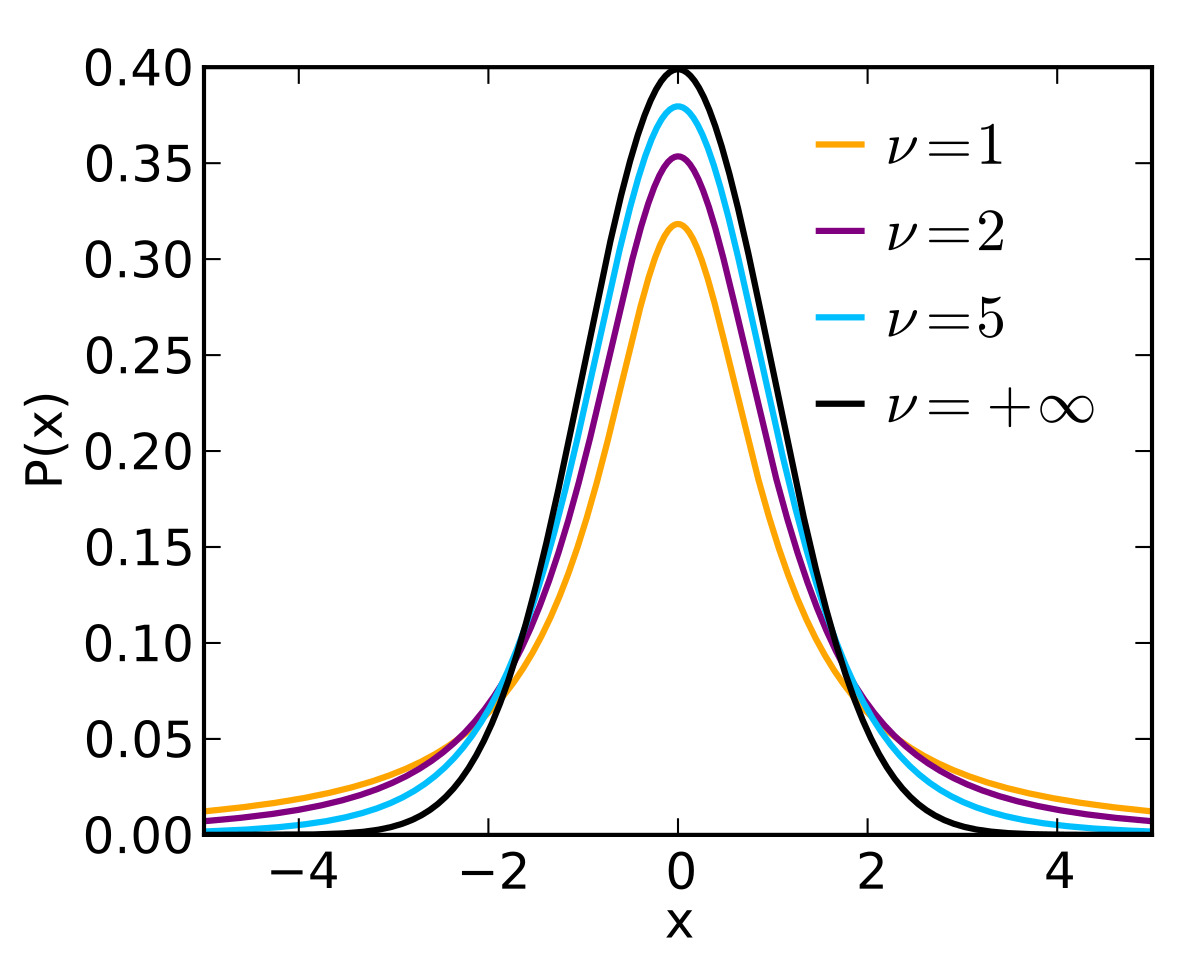
\includegraphics[width=\linewidth, height=4cm, keepaspectratio]{Pictures/distributions/Student_t_pdf.jpg}
            \caption{Student's t-Distribution: PDF}
        \end{figure}
    \end{minipage}
    \hfill
    \begin{minipage}{0.49\linewidth}
        \begin{figure}[H]
            \centering
            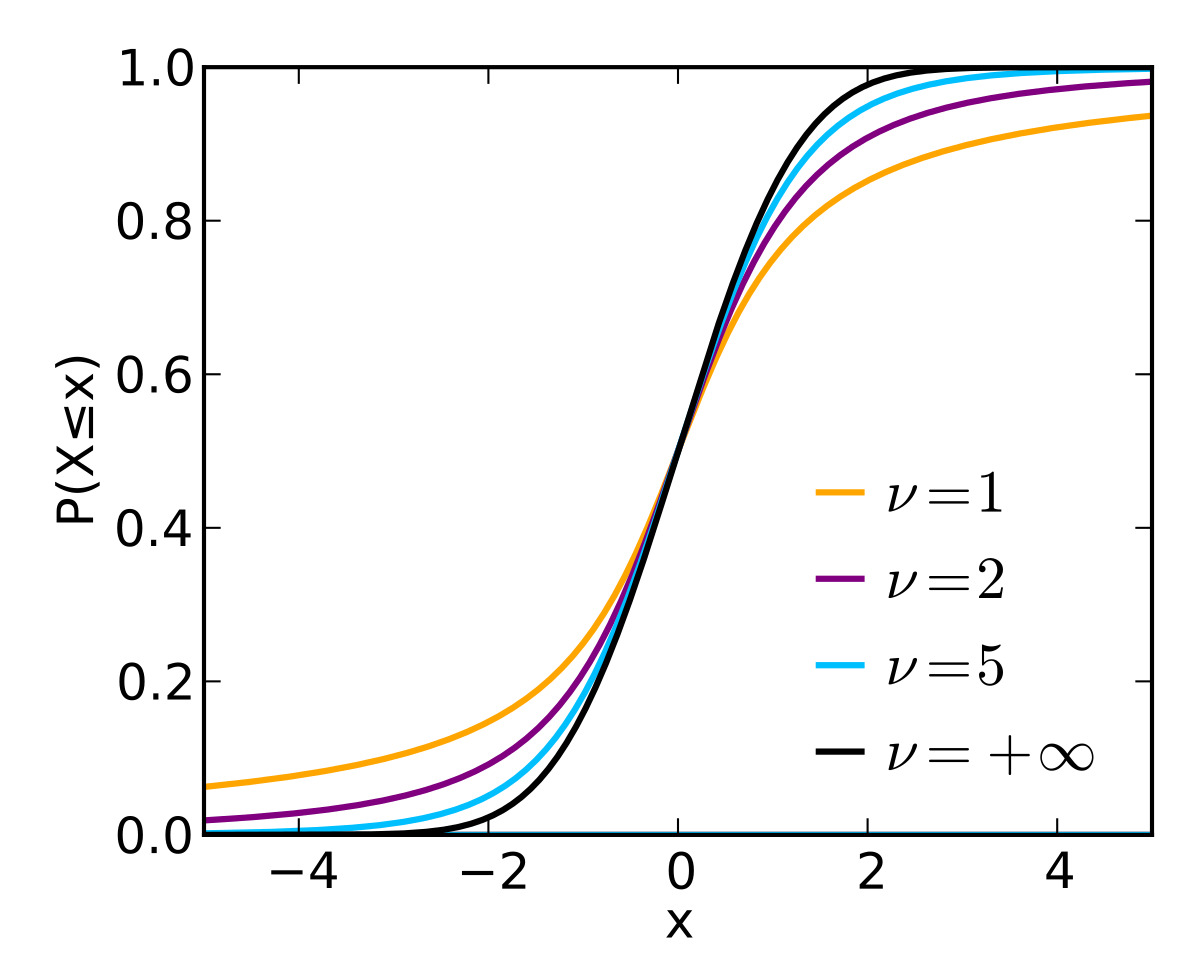
\includegraphics[width=\linewidth, height=4cm, keepaspectratio]{Pictures/distributions/Student_t_cdf.jpg}
            \caption{Student's t-Distribution: CDF}
        \end{figure}
    \end{minipage}
\end{table}

\begin{customTableWrapper}{2}
\begin{longtable}{|m{6cm}|p{9cm}|}
    \hline
    \customTableHeaderColor
    \multicolumn{2}{|c|}{\textbf{Student's t-Distribution - Info} \cite{wiki/Student_t-distribution}} \\
    \hline\endfirsthead

    \hline
    \customTableHeaderColor
    \multicolumn{2}{|c|}{\textbf{Student's t-Distribution - Info - contd.} \cite{wiki/Student_t-distribution}} \\
    \hline\endhead
    
    \hline\endfoot
    \hline\endlastfoot

    \textbf{Statistical parameters} & 
    ${ \ \nu >0\ }$ degrees of freedom (real, almost always a positive integer)
    \\ \hline
    
    \textbf{Support} &
    ${ \ x\in (-\infty ,\infty )}$
    \\ \hline

    \textbf{Probability Density Function (PDF)} &
    ${ \textstyle \ {\dfrac {\Gamma \left({\dfrac {\ \nu +1\ }{2}}\right)}{{\sqrt {\pi \ \nu \ }}\ \Gamma \left({\dfrac {\nu }{\ 2\ }}\right)}}\ \left(\ 1+{\dfrac {~x^{2}\ }{\nu }}\ \right)^{-{\dfrac {\ \nu +1\ }{2}}}\ }$
    \\[2ex] \hline
    
    \textbf{Cumulative distribution function (CDF)} &
    \tableenumerate{
        \item ${ {\begin{matrix}\ {\dfrac {\ 1\ }{2}}+x\ \Gamma \left({\dfrac {\ \nu +1\ }{2}}\right)\times \\[0.5em]{\dfrac {\ {{}_{2}F_{1}}\!\left(\ {\dfrac {\ 1\ }{2}},\ {\dfrac {\ \nu +1\ }{2}};\ {\dfrac {3}{\ 2\ }};\ -{\dfrac {~x^{2}\ }{\nu }}\ \right)\ }{\ {\sqrt {\pi \nu }}\ \Gamma \left({\dfrac {\ \nu \ }{2}}\right)\ }}\ \end{matrix}}}$ 

        \item[] where ${ \ {}_{2}F_{1}\!(\ ,\ ;\ ;\ )\ }$ is the hypergeometric function
    }
    \\ \hline

    \textbf{Mean} & 
    ${ \ 0\ }$ for ${ \ \nu >1\ }$, otherwise \textbf{undefined}
    \\[1ex] \hline

    \textbf{Median} & 
    $0$
    \\[1ex] \hline

    \textbf{Mode} & 
    $0$
    \\ \hline

    \textbf{Variance} &
    ${ \textstyle \ {\dfrac {\nu }{\ \nu -2\ }}\ }$ for ${ \ \nu >2\ }$, $\infty$ for ${ \ 1<\nu \leq 2\ }$, otherwise \textbf{undefined}
    \\[1ex] \hline

    \textbf{Skewness} &
    ${ \ 0\ }$ for ${ \ \nu >3\ }$, otherwise \textbf{undefined}
    \\ \hline

    \textbf{Excess kurtosis} &
    ${ \textstyle \ {\dfrac {6}{\ \nu -4\ }}}$ for ${ \ \nu >4\ }$, $\infty$ for ${ \ 2<\nu \leq 4\ }$, otherwise \textbf{undefined}
    \\[1ex] \hline

    \textbf{Entropy} &
    \tableenumerate{
        \item ${ \ {\begin{matrix}{\frac {\ \nu +1\ }{2}}\left[\ \psi \left({\frac {\ \nu +1\ }{2}}\right)-\psi \left({\frac {\ \nu \ }{2}}\right)\ \right]\\[0.5em]+\ln \left[{\sqrt {\nu \ }}\ {\mathrm {B} }\left(\ {\frac {\ \nu \ }{2}},\ {\frac {\ 1\ }{2}}\ \right)\right]\ {\scriptstyle {\text{(nats)}}}\ \end{matrix}}}$

        \item[] where
        \begin{enumerate}
            \item[] ${ \psi ()\ }$ is the digamma function
            
            \item[] ${ \ {\mathrm {B} }(\ ,\ )\ }$ is the beta function.
        \end{enumerate}
    }
    \\[1ex] \hline

    \textbf{Moment-generating function (MGF)} &
    undefined
    \\[1ex] \hline

    \textbf{Characteristic function (CF)} &
    \tableenumerate{
        \item ${ \textstyle {\dfrac {\ \left(\ {\sqrt {\nu \ }}\ \dabs{t}\ \right)^{\nu /2}\ K_{\nu /2}\left(\ {\sqrt {\nu \ }}\ \dabs{t}\ \right)\ }{\ \Gamma (\nu /2)\ 2^{\nu /2-1}\ }}\ }$ for ${ \ \nu >0\ }$
        
        \item[] ${ \ K_{\nu }(x)\ }$ is the modified Bessel function of the second kind
    }
    \\[1ex] \hline

    \textbf{Expected shortfall} &
    \tableenumerate{
        \item ${ \ \mu +s\ \left(\ {\frac {\ \nu +T^{-1}(1-p)^{2}\ \times \ \tau \left(T^{-1}(1-p)^{2}\right)\ }{\ (\nu -1)(1-p)\ }}\ \right)\ }$

        \item[] Where: 
        \begin{enumerate}
            \item ${ \ T^{-1}(\ )\ }$ is the inverse standardized Student t CDF
            \item ${ \ \tau (\ )\ }$ is the standardized Student t PDF
        \end{enumerate}
    }
    \\[1ex] \hline


\end{longtable}
\end{customTableWrapper}

\begin{enumerate}
    \item if $Z \sim \mathcal{N}(0,1)$ and $V_n^2 \sim \chi_n^2$ and $Z$ and $V_n^2$ are independent, $Z/(V_n/\sqrt{n})$ has a student t distribution

    \item Properties:
    \begin{enumerate}
        \item $x_p(f_t) = -x_{1-p}(f_t)$

    \end{enumerate}

    \item Confidence Interval:
    \begin{enumerate}
        \item If $x_p(f_t)$ is the $p$th quantile of the Student t-distribution with $n - 1$ degrees of freedom, the $1 - 2p$ confidence interval for $\mu$ (with $p < 0.5$) is:
        \[\left(
            \bar{X} - x_{1-p}(f_t)\dfrac{S}{\sqrt{n}},
            \hspace{0.2cm}
            \bar{X} + x_{1-p}(f_t)\dfrac{S}{\sqrt{n}}
        \right]\]

    \end{enumerate}

\end{enumerate}




















































